%----------------------------------------------------------------------------------------
%	PACKAGES AND OTHER DOCUMENT CONFIGURATIONS
%----------------------------------------------------------------------------------------
\documentclass[paper=a4, fontsize=11pt]{scrartcl} % A4 paper and 11pt font size
\usepackage[T1]{fontenc} % Use 8-bit encoding that has 256 glyphs
\usepackage{fourier} % Use the Adobe Utopia font for the document - comment this line to return to the LaTeX default
\usepackage[english]{babel} % English language/hyphenation
\usepackage{amsmath,amsfonts,amsthm} % Math packages
\usepackage{sectsty} % Allows customizing section commands
\allsectionsfont{\centering \normalfont\scshape} % Make all sections centered, the default font and small caps
\usepackage{fancyhdr} % Custom headers and footers
\usepackage{amsmath}
\usepackage{graphics}
\usepackage{graphicx}

\pagestyle{fancyplain} % Makes all pages in the document conform to the custom headers and footers
\fancyhead{} % No page header - if you want one, create it in the same way as the footers below
\fancyfoot[L]{} % Empty left footer
\fancyfoot[C]{} % Empty center footer
\fancyfoot[R]{\thepage} % Page numbering for right footer
\renewcommand{\headrulewidth}{0pt} % Remove header underlines
\renewcommand{\footrulewidth}{0pt} % Remove footer underlines
\setlength{\headheight}{13.6pt} % Customize the height of the header

\numberwithin{equation}{section} % Number equations within sections (i.e. 1.1, 1.2, 2.1, 2.2 instead of 1, 2, 3, 4)
\numberwithin{figure}{section} % Number figures within sections (i.e. 1.1, 1.2, 2.1, 2.2 instead of 1, 2, 3, 4)
\numberwithin{table}{section} % Number tables within sections (i.e. 1.1, 1.2, 2.1, 2.2 instead of 1, 2, 3, 4)

\setlength\parindent{0pt} % Removes all indentation from paragraphs - comment this line for an assignment with lots of text

%----------------------------------------------------------------------------------------
%	TITLE SECTION
%----------------------------------------------------------------------------------------

\newcommand{\horrule}[1]{\rule{\linewidth}{#1}} % Create horizontal rule command with 1 argument of height

\title{	
\normalfont \normalsize 
\horrule{0.5pt} \\[0.4cm] % Thin top horizontal rule
\huge ECE 760 Homework 2: kNN\\ % The assignment title
\horrule{2pt} \\[0.5cm] % Thick bottom horizontal rule
}

\author{Qihong Lu} % Your name
\date{\normalsize\today} % Today's date or a custom date

\begin{document}

\maketitle % Print the title

\section*{Question1}
Code: 
\begin{itemize}
	\item kNN\_alg.py: the main program that implements the standard kNN for multi-class classification and regression 
	\item util.py: the definitions of some constants and helper functions 
	\item kNN.py: run kNN algorithm, return test results
	\item kNN-select.py: run kNN algorithm, tune K by leave-one-out validation. Fit final model with the best K and return the test results 
\end{itemize}
 
\hfill 

Dependencies: 
\begin{itemize}
  \item pyhton 2.7 
  \item numpy 
  \item scipy 
  \item sys
\end{itemize}



%----------------------------------------------------------------------------------------
%	PROBLEM 2
%----------------------------------------------------------------------------------------
\newpage
\section*{Question2}

\textbf{For the yeast data set, draw a plot showing how test-set accuracy varies as a function of k. Your plot should show accuracy for k = 1, 5, 10, 20, 30.}
\begin{center}
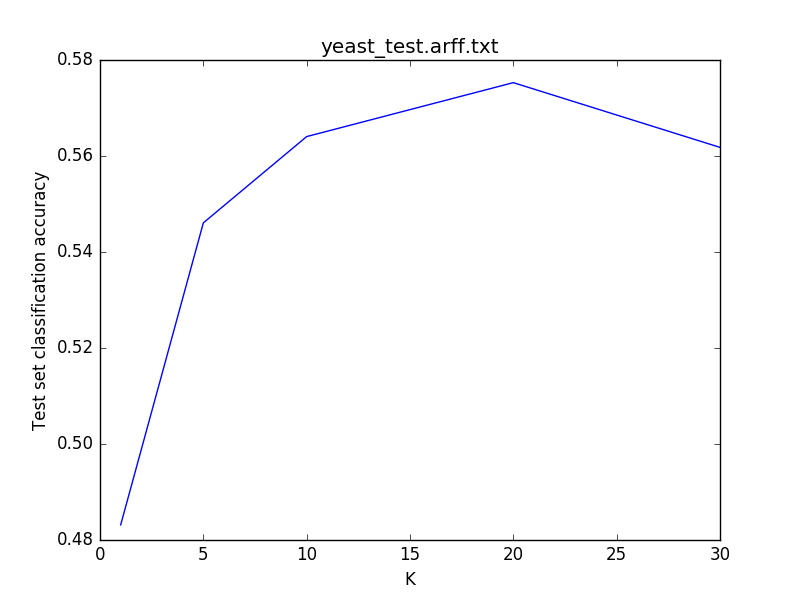
\includegraphics[scale=.55]{pics/hw2_2_1.png}
\end{center}

\textbf{For the wine data, draw a similar plot showing test-set mean absolute error as a function of k, for k = 1, 2, 3, 5, 10.}
\begin{center}
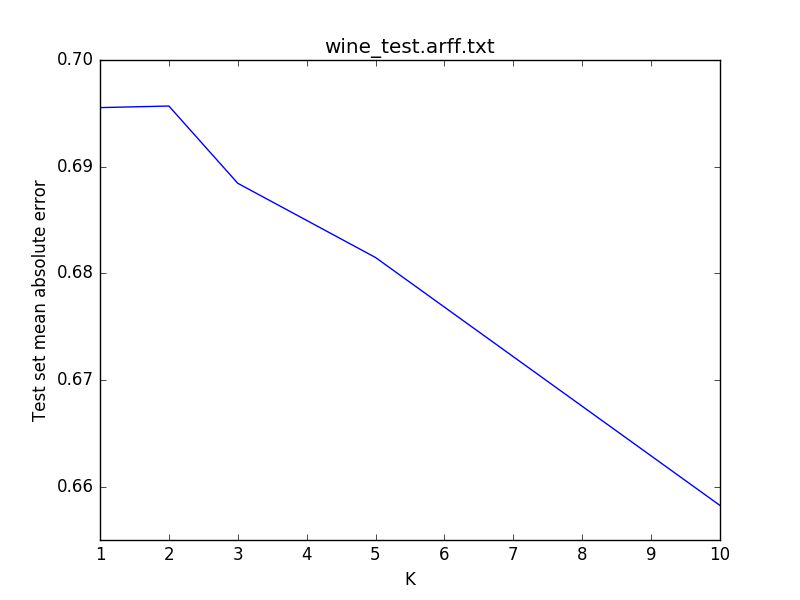
\includegraphics[scale=.55]{pics/hw2_2_2.png}
\end{center}


\newpage
\textbf{For the yeast data set, construct confusion matrices for the k = 1 and k = 30 test-set results. Show these confusion matrices and briefly discuss what the matrices tell you about the effect of k on the misclassifications.}

\begin{center}
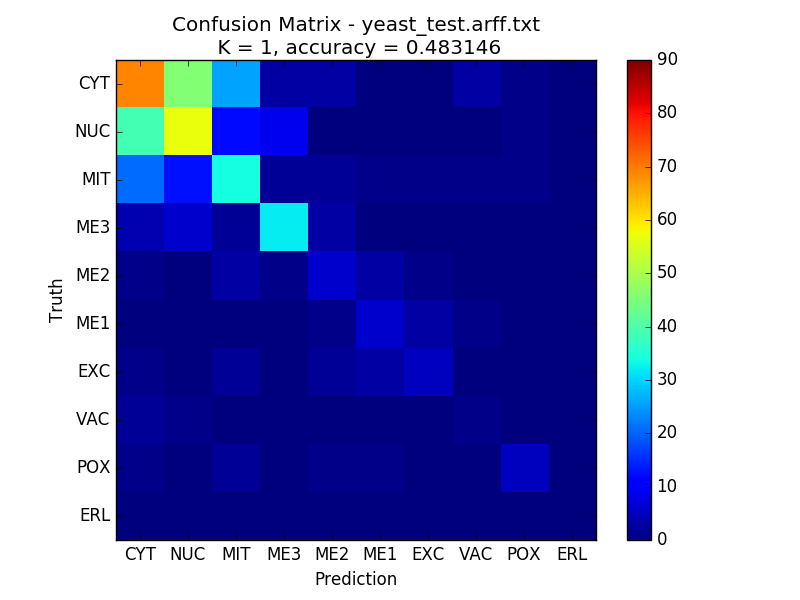
\includegraphics[scale=.6]{pics/hw2_2_3_1.png}
\end{center}

\begin{center}
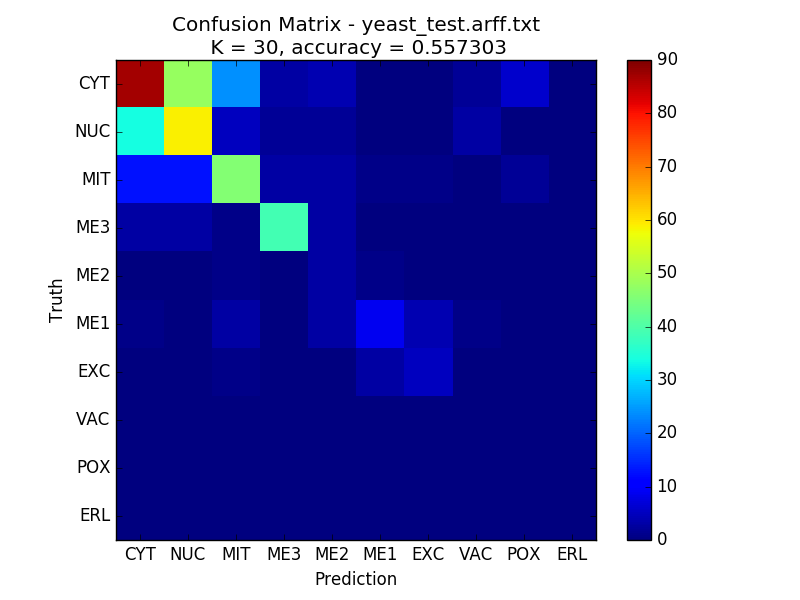
\includegraphics[scale=.6]{pics/hw2_2_3_2.png}
\end{center}

%----------------------------------------------------------------------------------------
%	PROBLEM 3
%----------------------------------------------------------------------------------------

\newpage
\section*{Question3}

%----------------------------------------------------------------------------------------
%	PROBLEM 4
%----------------------------------------------------------------------------------------
\textbf{Using the k-d tree and the training set displayed in the figure below, show how the nearest neighbor for $x^{(q)} = (7, 10)$ would be found.\\}

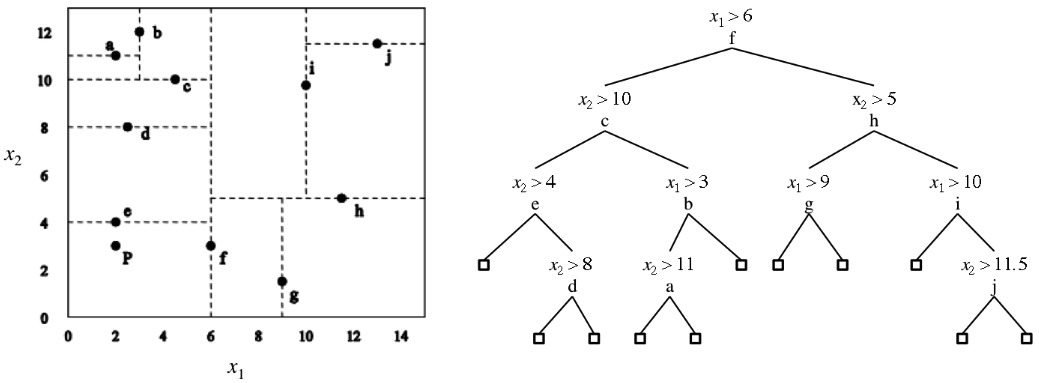
\includegraphics[scale=.4]{pics/question3.png}



\begin{center}
    \begin{tabular}{| l | l | l | l | p{6cm} |}
    \hline
    Action & Distance & Best Distance & Best Node & Priority Queue \\ 
    \hline    
    NA & $\infty$ & $\infty$ & NA & (f, 0) \\ 
    \hline    
    Pop f & 8 & 8 & f & (h, 0) (c, 1) \\ 
    \hline    
    Pop h & 8 & 10 & f & (i, 0) (c, 1) (g, 5)  \\
    \hline
    Pop i & 3 & 3 & i & (c, 1) (j, 3) (g, 5) \\
    \hline
    Pop c & 2 & 2 & c & (j, 3) (g, 5) \\
    \hline
    \end{tabular}
\end{center}
Therefore, the algorithm returns the node c. 
\end{document}